\documentclass{report}
\usepackage[utf8]{inputenc}


\usepackage[a4paper, total={6in, 8in}]{geometry}


\title{Entwiklung Algorithmus Obere Halswirbelsäule}
\author{Lukas Hörnig}
\date{Oktober 2017}

\usepackage[square,sort,comma,numbers]{natbib}
\usepackage{graphicx}
\usepackage[hidelinks]{hyperref}
\usepackage{gensymb}

\begin{document}
\section{Klinische Instabilität}
\begin{figure}[h]
        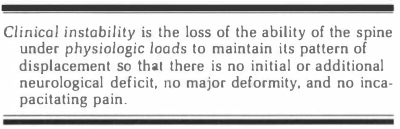
\includegraphics[width=8cm]{Instability.png}
\end{figure}

\section{Auswahl der Werte}
\subsection{Atlanto-occipitale Dislokation}
\paragraph{Distraktion, Trankslation}
% Doppelte Bewertung von AOD durch CS/CG und BDI?
% Werte und Studien zu BAI
Bevorzugung des Basion-Dens-Inteval (BDI) und Basion-posterior axial line Interval (BAI) \cite{WHOLEY1958,Harris1994,Harris1994a} über den Methoden Power's Ratio \cite{Powers1979} und X-Lines \cite{Lee1987}, durch Überlegenheit in Sensitivität, Spezifität, positiv prädiktivem und negativ prädiktivem Wert sowie in der Anwendbarkeit durch Lesbarkeit und Simpliziät. \cite{Deliganis2000,Fisher2001,Harris1994,Dziurzynski2005,Radcliff2010,Chang2009,Chaput2011,Bono2007}\\

\paragraph{Kompression}
Eine Kompressionsfraktur im Rahmen eine Jefferson Fraktur des Atlas \cite{Jefferson1919,Jefferson1927} mit begleitender Instabiltät durch Ruptur des Ligamentum transversale (TAL) wird durch einen erhöhten Wert des Lateral Mass Displacemnts (LMD) abgebildet.
\subsection{Atlantoaxiale Dislokation}

Zur Beurteilung der Stabilität des Gelenkkomplexes zwischen Atlas und Axis werden verschiedene Werte der knöchernen Strukturen herangezogen um Verletzungen des für die Stabilität verantwortlichen Bandapparates zu beurteilen. \cite{Dvorak1988,Lopez2015,White1990}

\paragraph{Distraktion}
Durch Distraktion entstandene Verletzungsmuster manifestieren sich zwischen Atlas und Axis im ligamentär im Bereich der Gelenkkapsel zwischen den Processus articularis und den Ligamenta cruciforme.\\
Ein erweiterter Abstand der Gelenkflächen gibt in der Computertomographie den Hinweis auf eine Ruptur der Stabilität gebenden Bandstrukturen. \cite{Gonzalez2004,Chaput2011,Radcliff2010}

\section{Harris Measurements}
\subsection{Definiton}
\paragraph{Basion-Dens-Interval}

\begin{figure}[h]
        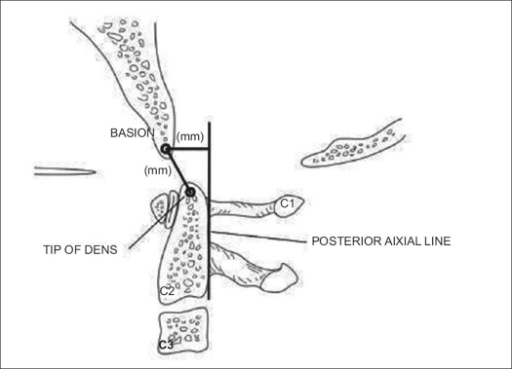
\includegraphics[width=8cm]{BDI.png}
\end{figure}

Länge der kürzesten Distanz zwischen dem Mittelpunkt des Basion und der Spitze des Dens in sagitaler Mittelininerekonstruktion in Millimetern.


\paragraph{Basion-posterior axial line - Interval}
Länge der kürzeste Distanz zwischen einer rechtwinkligen Linie vom Basion zu einer Verlängerung der Linie an der Hinterkante des vorderen Axisrings in sagitaler Mittelininerekonstruktion in Milimetern.

\subsection{Statistik}
Das BDI zeigt über die Altersgruppen und Geschlechter keine nennenswerte Instabilität \cite{Chaput2011} und wurde schon bezüglich Normwerte und pathologischer Abweichung ausgiebig untersucht.
\cite{Radcliff2010,Radcliff2012,Chang2009,Harris1994,Harris1994a,Chaput2011,Rojas2007,Gonzalez2004,Gonzalez2004a,Dziurzynski2005,Bono2007}. 



\paragraph{Validität}
% Resultiert aus Dislokation Instabilität??
Sowohl für die Sensibilität als auch für die Spezifität bezüglich des BDI für Atlanto-occipitale Dislokation und daraus resultierender Instabilität zeigen sich eine hohe Güte \cite{Dziurzynski2005}.

\paragraph{Reliabiliät}
% Hier fehlen noch die genauen Berechnungsformen und Kappa werte PDF-Chapter 6
Der BDI zeigt sich sowohl bezüglich Intra- und Interobserver Reliabiliät eine sehr hohe Güte \cite{Chaput2011,Dziurzynski2005,Harris1994,Harris1994a}, welche durch stabile Verhältnisse und verbesserte Bildgebung, sowie deren Lesbarkeit, welche durch verlässliche Darstellung der benötigten anatomischen Landmarken garantiert werden \cite{Dziurzynski2005,Radcliff2010}.


\subsection{Patholgischer Wert}
% Auswertung Graphisch wie in \cite{Woods2017}
Ab einem BDI von über 10 mm und/oder einem BAI von mehr als 12 mm sollte von einer Instabilität durch Atlanto-occipitale Dislokation ausgegangen werden.


\subsection{Anwendbarkeit}
Die Anwendbarkeit wird bei Messung an CT-Bildgebung durch hochaufgelöste, überlagerungsfreie Darstellung für erfahrene Anwender der Technik sehr zuverlässig und in fast allen Fällen möglich gemacht \cite{Dziurzynski2005,Radcliff2010}. 


\section{Laterl Mass Intervall}
\subsection{Definition}

\begin{figure}[h]
        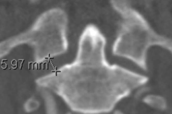
\includegraphics[width=8cm]{LMI.png}
\end{figure}
\subsection{Definition}

\section{Statistik}
\subsection{Validität}
Bezüglich der Validität konnten nur Studien gefunden werden, welche einen Hinweis auf Instabilität und eine Implikation für magnettomographische Bildgebung durch erhöhte Werte der LMI geben. \cite{Chaput2011,Gonzalez2004,Radcliff2010}


\subsection{Reliabiliät}
% Hier fehlen noch die genauen Berechnungsformen und Kappa werte PDF-Chapter 6
Das LMI zeigt bezüglich Intraobserver Reliabiliät eine sehr hohe Güte und bezüglich der der Interrater Reliabiliät gute Werte \cite{Chaput2011}, welche durch stabile Verhältnisse und verbesserte Bildgebung, sowie deren Lesbarkeit, welche durch verlässliche Darstellung der benötigten anatomischen Landmarken garantiert werden \cite{Radcliff2010}.

\subsection{Stabilität}
Das LMI zeigt über Altersgruppen und Geschlechter hinweg eine statistisch signifiktante Instabilität \cite{Chaput2011}




\section{Lateral Mass Displacement}
\begin{figure}[h]
        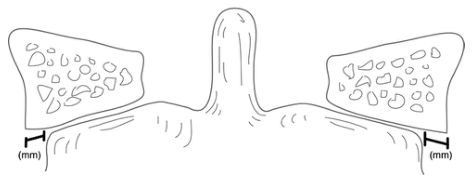
\includegraphics[width=8cm]{LMD.png}
\end{figure}
\subsection{Definition}
Das Lateral Mass Displacement wird als Distanz zwischen dem am weitesten lateralen Anteil des Processus articularis des Atlas und des Axis in Milimetern gemessen.
Zur Darstellung wird ein coronarer Schnitt auf Höhe der Zentrums der Massa lateralis des Atlas gewählt.
\cite{Bono2007}
% Korrekten Plural von Massa lateralis herausfinden
% Milli oder Mili?
% Coronar oder Koronar?

\subsection{Statistik}


\paragraph{Validität}
Durch biomechanische Kadaver Studien \cite{Woods2017,Spence1970} und klinsche Bildgebung verschiedenster Art \cite{Radcliff2010,Perez_Orribo_2016,Heller1993,Radcliff2013} wurde ein Zusammenhang zwischen dem LMD und einer Ruptur des Ligamentum transversale (TAL) festgestellt.\\
Durch statistische und klinische Analyse ergibt sich jedoch für die Schnibildgebung ein signifikant \cite{Woods2017} geringer Wert als ursprünglich von angenommen. \cite{Spence1970} 
Die aktuelle Annahmen decken sich mit der Klassifikation nach Dickman \cite{Dickman1996}. 


\paragraph{Reliabiliät}
Es konnten keine Studien zur Intra- bzw Interobserver Reliabiliät gefunden werden.


\subsection{Pathologischer Wert}
Ab 3,8 Millimetern sollte eine Ruptur des TAL bis zum Ausschluss durch magnettomographische Bildgebung angenommen werden \cite{Woods2017,Radcliff2013}.



\bibliography{../literatur}
\bibliographystyle{dinat}
\end{document}
